\chapter{散乱角度}\label{cha:angle}
\section{光生成反応の散乱角度}
図\ref{fig:angle1}のように実験室系での$\mu$の散乱角$\theta$,中間状態$\gamma^*N$系の散乱角$\phi$を定義する.
\begin{figure}[H]
    \centering
    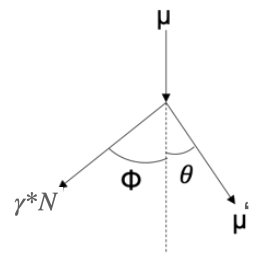
\includegraphics[height=4cm]{img/angle_diagram.png}
    \caption{散乱角$\theta, \phi$の定義}
    \label{fig:angle1}
\end{figure}

\subsection{$\theta$の取る値}
図\ref{fig:angle2}のような運動学変数を考える.
\begin{figure}[H]
    \centering
    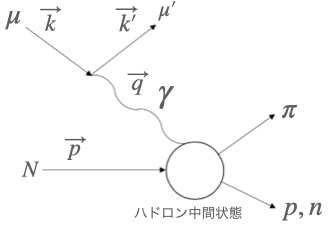
\includegraphics[height=4cm]{img/diagram_3momentum.png}
    \caption{運動学変数の定義}
    \label{fig:angle2}
\end{figure}
各値に対して以下のような定義を行う.
このとき, $\mu$の進行方向の運動量成分を
$p_\parallel$, 垂直方向の成分を $p_\perp$ として, 4元運動量を
$p = (E, p_\parallel, p_\perp) $とあらわすと, 各粒子の運動量は以下の通りとなる.
\begin{equation}
    k = (E_\mu , p_\mu,0)
\end{equation}
\begin{equation}
    k' = (E'_\mu, p'_\mu \cos\theta, p'_\mu \sin\theta)
\end{equation}
\begin{equation}
    p = (m_N, 0, 0)
\end{equation}
\begin{equation}
    q = k-k'=(E_\mu - E'_\mu, p_\mu-p'_\mu \cos\theta, -p'_\mu \sin\theta)
\end{equation}
また, $Q^2$は$q$を用いることにより式\ref{eq3_1}のように表せる.
\begin{equation}
    \label{eq3_1}
    Q^2 = -q^2 = 2E_\mu E'_\mu -2m^2_\mu-2p_\mu p'_\mu \cos\theta
\end{equation}
式\ref{eq3_1}を$\theta$について解く.

$E'_\mu = E_\mu(1-y), p'_\mu = \sqrt{E'^2_\mu - m^2_\mu}$
を用いて$E'_\mu, p'_\mu$を消去すると, 
\begin{eqnarray}
    \theta & = &\arccos \left( \dfrac {2E_\mu E'_\mu -2m^2_\mu-Q^2}{2p_\mu p'_\mu} \right) \\
    & = & \arccos \left(\dfrac{-Q^2-2m^2_\mu+2E^2_\mu(1-y)}{2\sqrt{E^2_\mu-p^2_\mu}\sqrt{E^2_\mu(1-y)^2-m^2_\mu} }  \right)
\end{eqnarray}
この$\theta$は図\ref{fig:angle3}のようになる.
\begin{figure}[H]
    \centering
    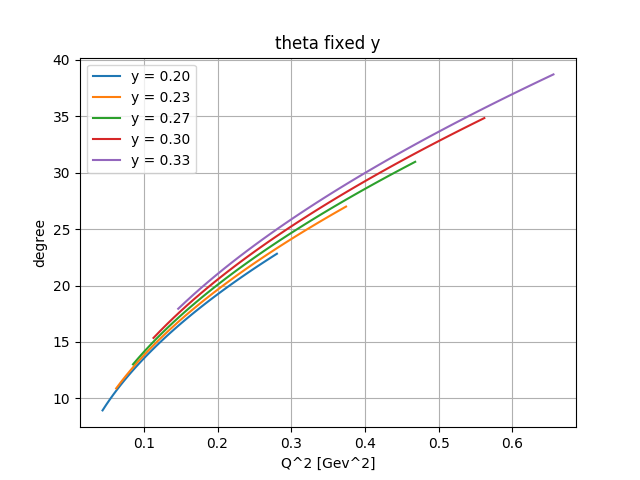
\includegraphics[height=5cm]{img/theta_degree_y_fixed.png}
    \caption{$\mu$の散乱角$\theta$の$Q^2$依存性}
    \label{fig:angle3}
\end{figure}
$\theta$はyが小さくなると小さくなる.また$Q^2$が小さくなると小さくなる.
$\theta$は$\theta=[10^\circ,40^\circ]$の範囲であることがわかる.

\subsection{$\phi$の取る値}
\begin{equation}
    \vec{p_\mu} \cdot \vec{p_W} = |p_\mu| |p_W| \\ \cos\phi
\end{equation}
から
\begin{equation}
    \phi = \arccos \left( \dfrac{yE^2_\mu + \dfrac{Q^2}{2}} {\sqrt{(E^2_\mu - m^2_\mu)(y^2E^2_\mu+Q^2)}} \right)
\end{equation}
$\phi$は図\ref{fig:angle4}のようになる.
\begin{figure}[H]
    \centering
    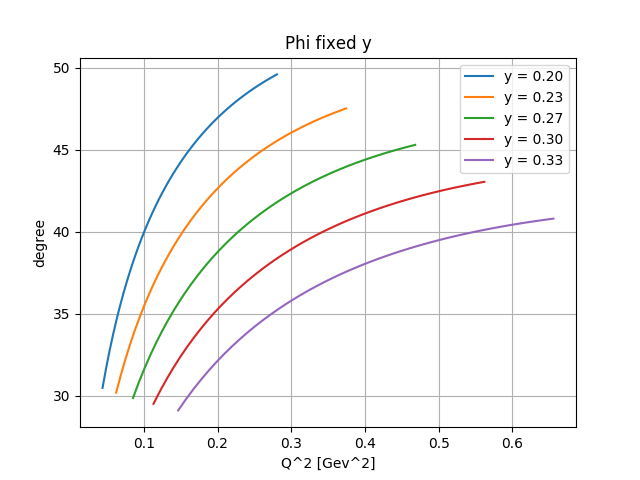
\includegraphics[width=8cm]{img/Phi_degree_fixed_y.png}
    \caption{中間状態の散乱角$\phi$の$Q^2$依存性}
    \label{fig:angle4}
\end{figure}
中間状態の散乱角$\phi$はyが小さくなると大きくなる.また, $Q^2$が小さくなると小さくなる.
$\phi$は$\phi = [30^\circ, 50^\circ]$ の範囲にあることがわかる.

\section{\texorpdfstring{$\gamma N$の崩壊で生成される$\pi, p$について}{LG}}
\subsection{$\gamma^* N$から生成される$\pi,p$の静止系での運動量とエネルギー}
\begin{figure}[H]
    \centering
    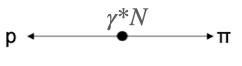
\includegraphics[width=6cm]{img/rest_middle_situation.png}
    \caption{静止した$\gamma^* N$から生成される$\pi,p$}
    \label{fig:angle5}
\end{figure}
図\ref{fig:angle5}のような静止した$\gamma^* N$を考える.
$m_W = 1.08 \ $GeV, $E_\mu = 1.5 \ $GeVを仮定する.
この仮定から$y = 0.2$で$Q^2 \approx 0.28 \ \mathrm{GeV^2}$となる.
それぞれの粒子が持つエネルギーと運動量を導出する.
エネルギー保存則から
\begin{equation}
    \label{eq3_3}
    E_W = E_\pi + E_p
\end{equation}
運動量保存則から
\begin{equation}
    \label{eq3_4}
    p_p = p_\pi
\end{equation}
式\ref{eq3_3}, \ref{eq3_4}から
\begin{eqnarray}
    E_W  & =  & E_\pi + \sqrt{m_p^2 + p_p^2} \\
    & = & E_\pi + \sqrt{m_p^2 + p_\pi^2} \\
    & = & E_\pi + \sqrt{m_p^2 + E_\pi^2 - m_\pi^2}
\end{eqnarray}
$E_\pi$について解くと
\begin{equation}
    E_\pi = \dfrac{E_W ^2 + m_\pi ^2 - m_p ^2}{2E_W}
\end{equation}
同様に$E_p$を導出すると, 
\begin{equation}
    E_p = \dfrac{E_W ^2 + m_p ^2 - m_\pi ^2}{2E_W}
\end{equation}
運動量は関係式
\begin{equation}
    p^2 = \sqrt{E^2 - m^2}
\end{equation}
から見積もる.
$E_W = 1.15 \ $GeV, $m_p = 0.938 \ $GeV, $m_\pi = 0.138 \ $GeVとして代入すると, 
$E_π = 200.7 \ $MeV, $E_p = 949.0 \ $ MeV , $p_π = p_p = 145.8 \ $ MeVとなる.

\subsection{実験室系にブーストされた$\gamma^* N$から生成される$\pi,p$の運動量}
\begin{figure}[H]
    \centering
    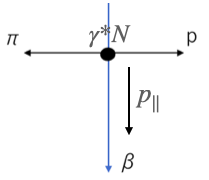
\includegraphics[height=3cm]{img/boost_middle_situation.png}
    \caption{実験室系にブーストされた$\gamma^* N$から生成される$\pi,p$}
    \label{fig:angle6}
\end{figure}
実験室系にブーストされた$\gamma^* N$を考える.
ローレンツ変換の式\ref{eq3_5}を用いて運動量を計算する.
\begin{equation}
    \label{eq3_5}
    \left(\begin{array}{c}
            E^* \\
            p^*_\parallel
        \end{array}\right)
    =\left(\begin{array}{cc}
            \gamma \ \ -\gamma \beta \\
            -\gamma \beta  \ \  \gamma
        \end{array}\right)
    \left(\begin{array}{c}
            E \\
            p_\parallel
        \end{array}\right)
\end{equation}
ここで
\begin{eqnarray}
    \beta = \dfrac{p_W}{E_W} = \dfrac{p_\gamma + p_p}{E_\gamma + E_p} = 0.24
\end{eqnarray}

\begin{eqnarray}
    \gamma = \dfrac{1}{\sqrt{1 - \beta^2}} \approx 1.03
\end{eqnarray}
となる.
このことから中間状態はあまりブーストされないことがわかる.

\begin{figure}[H]
    \centering
    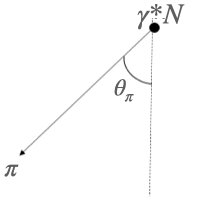
\includegraphics[height=5cm]{img/theta_pi.png}
    \caption{静止した$\gamma^* N$から出てくる$\pi$の散乱角}
    \label{fig:angle7}
\end{figure}

静止した$\gamma^* N$系から$\pi$が出てくる角を$\theta_\pi$として, 
$\pi$の運動量について考える.
$\gamma^* N$系の進行方向に対して垂直な運動量成分を$p_{\pi \perp}$, 平行な運動量成分を$p_{\pi \parallel}$とすると以下の式が成り立つ.

\begin{eqnarray}
    p_{\pi \parallel} = p_\pi  \cos\theta \\
    p_{\pi \perp} = p_\pi \sin\theta
\end{eqnarray}

\section{\texorpdfstring{実験室系にブーストされた$\gamma^* N$から生成される$\pi$の散乱角}{LG}}
ローレンツ変換の式から$p'_{\pi \parallel}$を導出し, $p_{\pi \perp} = p'_{\pi \perp}$であるから, 
\begin{equation}
    p'_\pi = \sqrt{p'^2_{\pi \parallel} + p'^2_{\pi \perp} }
\end{equation}
$\theta_\pi$が等方的に出た時にブーストされた$\gamma^* N$から出てくる$\pi$の角度を$\phi_\pi$とすると,
\begin{equation}
    p'_{\pi \parallel} = p'_\pi \cos{\phi_\pi}
\end{equation}
よって, 
\begin{equation}
    \phi = \arccos{\dfrac{p'_{\pi \parallel}}{p'_\pi}}
\end{equation}
$\theta_\pi$が等方的に出るとして$\phi_\pi$の分布は\ref{fig:angle8}のようになった.
\begin{figure}[H]
    \centering
    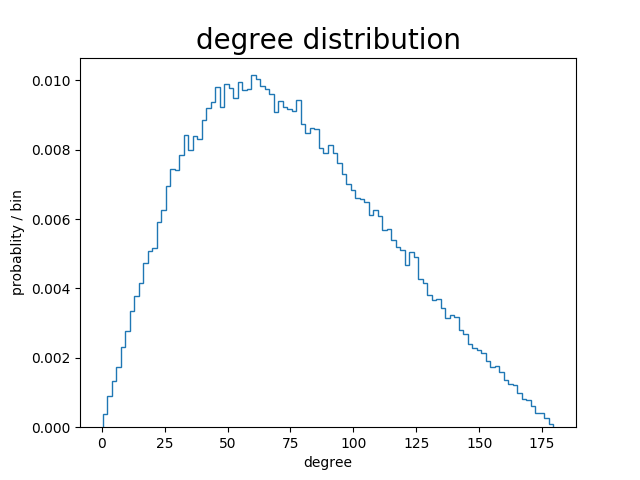
\includegraphics[height=7cm]{img/degree_distribution.png}
    \caption{$\pi$の角度分布}
    \label{fig:angle8}
\end{figure}
$\phi_\pi$は60°付近にピークを持つため主に進行方向成分が大きいが, 
同時に横方向の運動量成分も大きいことがわかる.